
\subsection{Parameter range modification for the biophysical candidates in the model. }
Computational models are a powerful tool to assess the source of neural dynamics where all variables involved are accessible. By considering membrane potential recordings alone, it is difficult to understand the contribution of the biophysical candidates in the underlying dynamics shaping the action potential. While it is specially hard to carry out experiments using chemical and/or electrophysiological techniques to selectively block or compensate channels to mimic the observed CW-NIR laser effect, the simultaneous accessibility to all the variables in a model provides a unique tool to dissect the contribution of all biophysical candidates. Thus, to further explore the source of the experimentally observed CW-NIR effect, we analyzed the spike generation dynamics in three different conductance-based models assessing the change in the most likely candidates to be affected by the laser stimulation: modulation of membrane capacitance and ionic channels. More specifically, we modulated (i) the capacitance and the conductance of the active ionic channels --$I_{Na}$ and $I_{K}$-- in the standard Hodgkin-Huxley (HH) model \parencite{hodgkin_quantitative_1952}; (ii) the conductance of ionic channels --$I_{NaP}$,~$I_{NaT}$,~$I_{D}$,~$I_{A}$,~$I_{HVA}$,~$I_{LVA}$-- and capacitance in a \textit{Lymnaea stagnalis} CGC neuron model with a shoulder shape waveform \parencite{vavoulis_balanced_2010}; and (iii) the capacitance in a two-compartment model --where the fast and slow dynamics are segregated-- in a \textit{Lymnaea stagnalis} buccal ganglion neuron (N3t) model \parencite{vavoulis_dynamic_2007}. The implementation of these models is available in the open-source model library Neun \href{https://github.com/GNB-UAM/neun}{github.com/GNB-UAM/Neun} and the code for the simulations can be accessed in \href{https://github.com/GNB-UAM/Garrido-Pena_Modulation-neural-dynamics-by-CW-NIR-stimulation}{github.com/GNB-UAM/Garrido-Pena\_Modulation-neural-dynamics-by-CW-NIR-stimulation}.

The model parameters were modulated to investigate and compare their effect to that of the CW-NIR laser stimulation on the neurons, and to evaluate the interrelationship between the observed changes. To identify changes in the spike dynamics similar to those observed under the CW-NIR laser illumination, in this section we covered a complete range of values in the parameter space of each biophysical candidate. The criteria for driving the parameter exploration were the preservation of tonic spiking in the activity and the assessment of a realistic range of values.
As our initial hypothesis did not assume that the CW-NIR laser effects were exclusively photo-thermal, model parameter changes were applied with no temperature description. Further down in Sec. \ref{sect:temperature model} we present a detailed study considering the temperature dependency of the biophysical candidates. 

\begin{figure}[hbt!]
	\centering
	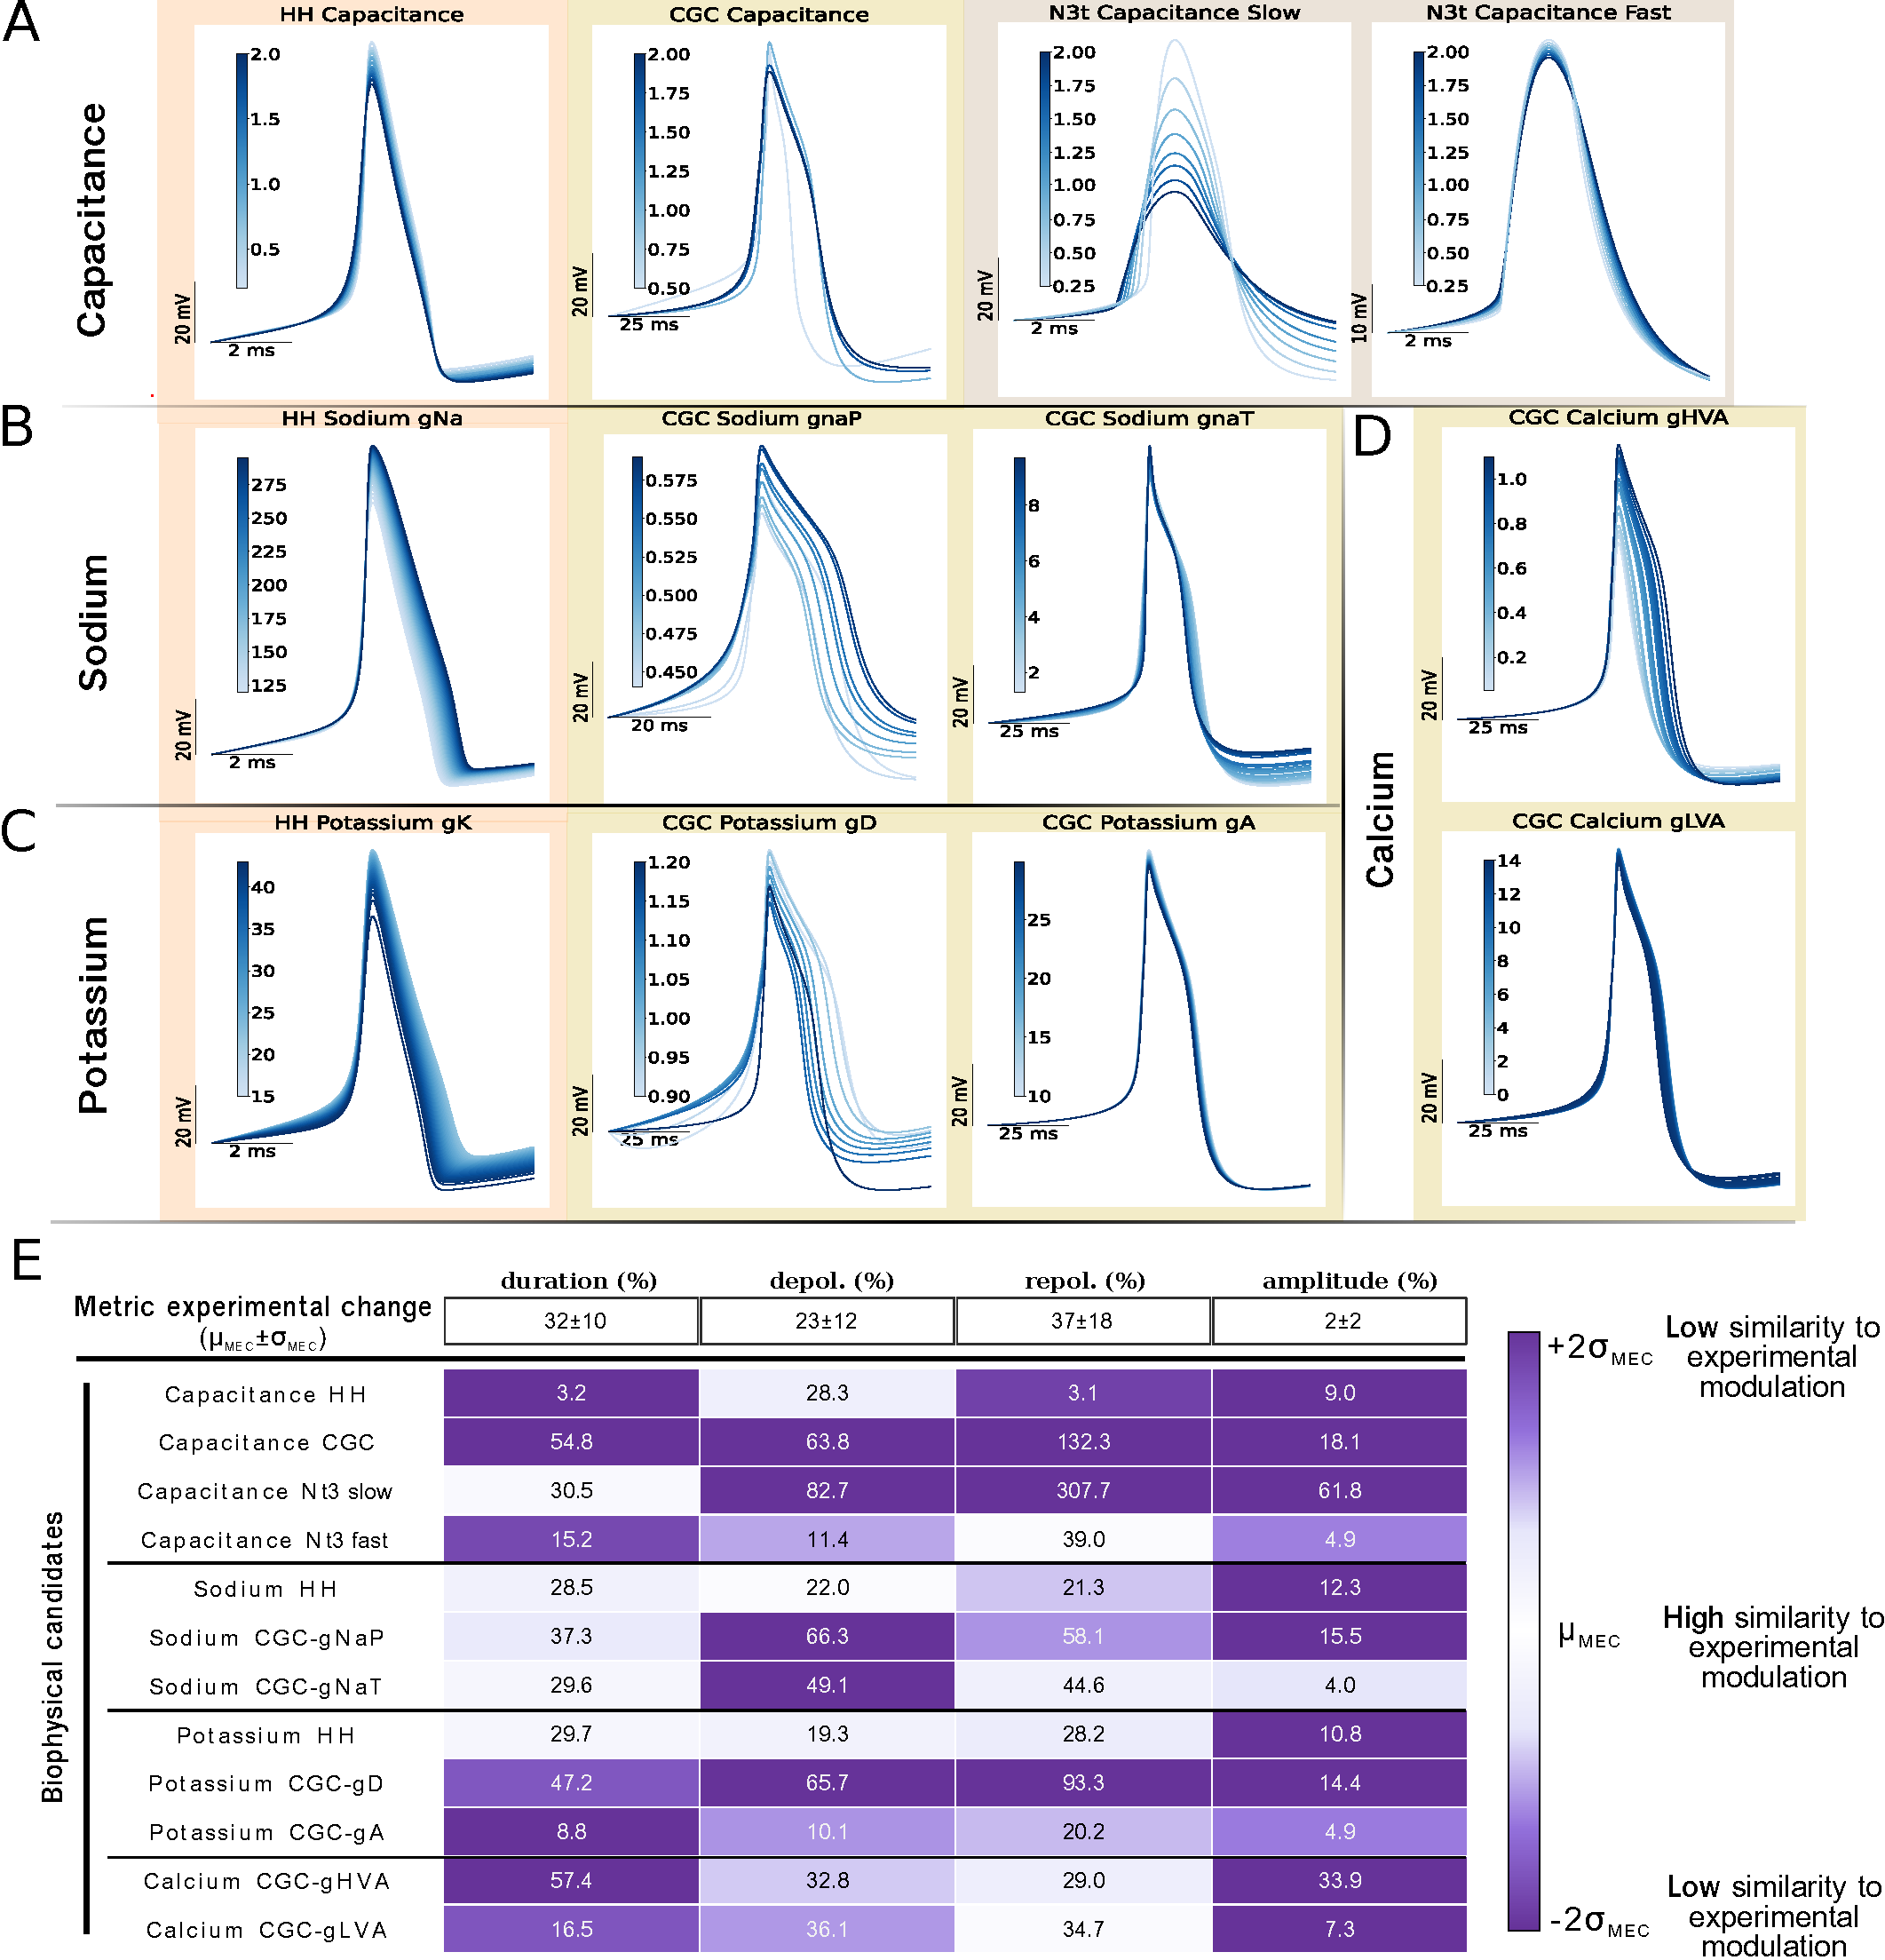
\includegraphics[width=0.8\textwidth]{img/laser/Figure4.pdf}
	
	\caption{Modeling study of the CW-NIR laser stimulation effects due to isolated biophysical changes that alter the spike waveform. Panels A, B, C and D: Superposition of spike waveforms in each model by modulating a single biophysical candidate. The background colors correspond to each simulated model. In Panel A, the capacitance is changed for the HH and CGC neuron models, and in the two compartments for the N3t neuron model. Panel B shows the spike waveforms changing the conductances of $Na$ channel currents: $I_{Na}$ from the HH-model, $I_{NaP}$ and $I_{NaT}$, from the CGC-model. Panel C, displays the modulation of $K$ conductances in ionic currents: $I_{K}$ in the HH-model and $I_{D}$ and $I_{A}$ for the CGC-model (from left to right). Panel D shows the modification of the calcium current conductances in the CGC-model ($I_{HVA}$ and $I_{LVA}$). Table in panel E represents the quantification of the changes in the spike metrics when tuning each parameter for every model. Each cell contains the waveform change normalized to the maximum. The color gradient represents similarity based on the standard deviation of the normalized experimental change. Dark purple corresponds to low similarity ($2\sigma_{\textrm{MEC}}$ or larger) and white to high similarity. The quantified experimental reference (MEC) is annotated in the first row of the table.}
	\label{fig:continuous_model}
\end{figure}

The results of this study are shown in Fig. \ref{fig:continuous_model}. The analysis for each model is sorted by the explored biophysical candidate --capacitance, sodium channels, potassium channels and calcium channels--. Thus, panels A, B, C and D show the superposition of all spike waveforms from the simulations for the range of explored model parameter values of each candidate. The table in Panel E represents how well the different model candidates reproduce the observed experimental effect. For each metric and biophysical candidate, there is a percentage of change in the model calculated as the change from minimum to maximum normalized with the maximum value (analogously to the quantification in Fig. \ref{fig:continuous_results_panel}, see also Sec. \ref{sect:statistical_analysis}). The background color in each cell represents the ability of each model parameter modulation to produce results similar to the change in the experimental results. The color gradient (represented in the color bar) takes as reference the mean of the metric experimental change (MEC) quantification, considering the range of $(\mu_{\textrm{MEC}}\pm2\sigma_{\textrm{MEC}})$ (see Sec. \ref{sect:statistical_analysis}). The mean change and its standard deviation were computed as the normalized difference between mean values for each control and laser experimental pair for all experiments. These reference values are shown for each metric in the first row of the table in panel \ref{fig:continuous_model}E to compare them with the model results. Thus, dark purple corresponds to values two times the STD of the mean over or under the mean, and white represents the mid point between those two values, i.e., high similarity to the experimental modulation. For example, in the case of Capacitance in the HH model, the change in duration was minimal 3.2\%, while the mean change in the experimental observation was 32\%, this color is then represented in dark purple, since 3.2\% is not in the defined range (32±20). On the other hand, the change in depolarization slope for this model (28.3\%) is depicted in light purple, since it is in the defined range and close to the mean metric experimental change (23±12).


\subsubsection{Change in Capacitance}
Capacitance has been one of the most discussed biophysical candidates to be affected by IR laser illumination \parencite{shapiro_infrared_2012, shapiro_correction_2017,cayce_infrared_2014, plaksin_thermal_2018}. A change in capacitance has a direct effect on the spiking frequency and exerts a global modulation on all ionic currents, so many studies have discussed this change both experimentally and theoretically.
Here we explored the CW-NIR modulation of capacitance in three different conductance-based models: in the Hodgkin-Huxley model, used in other studies, in the CGC-Vavoulis model, which presents a variety of channels and in the N3t-model, which is the only one with more than one compartment and, thus, has two distinct capacitance values. 

Figure \ref{fig:continuous_model}A displays the waveforms of each simulation. In the case of the HH-model, there was a mild change in duration, mainly caused by the depolarization modulation, and a change in amplitude larger than what was observed experimentally. The CGC-model exhibited a similar tendency to the HH-model but with an extreme case at a low value of capacitance $0.5 \mu F/cm^2$, where moderated changes in depolarization and amplitude were combined with a large change in the repolarization, and consequently in the duration. This modulation made capacitance a better candidate for reproducing the experimental results in the case of the CGC neuron, preserving the metrics' change interrelations, i.e., the combination of a minimal change in amplitude and a large change in duration, together with a larger change in repolarization than in depolarization slope. In the N3t neuron, we can see contrasting results for the two different compartments. In the compartment containing slow currents, the change in amplitude was the most striking, seemingly conditioned by both slopes. In the case of the fast current compartment the main change was observed in repolarization rather than depolarization, which is more similar to the experimental outcome. 

These results are quantified in the table in Fig. \ref{fig:continuous_model}E. The HH-model showed a change comparable to the experimental one only for the depolarization slope. The CGC-model reached plausible values in terms of the interrelation between metrics (large change in duration generated by a larger change in repolarization than in depolarization slope), but it exceeded the experimental references. The change in amplitude was larger than seen in the experimental results for most parameters (dark purple). It is especially clear in the case of the two-compartment model (N3t neuron), in which the modulation of capacity in the slow compartment resulted in a large change in amplitude. In contrast, the small change in amplitude in the fast compartment was the most similar value with respect to the experimental results (light purple).

By changing the capacitance, we achieved some of the expected changes, but achieving the desired results for all four metrics simultaneously was not possible. Therefore, modulating capacitance alone does not reproduce the experimentally observed effects, especially regarding the combined change, e.g., large change in repolarization and small change in amplitude, larger change in repolarization than in the depolarization. It was only when the fast compartment of N3t was modified that relations between these four metrics matched the above relationships. But note that changing the capacitance in the slow compartment is equivalent to changing several ionic currents simultaneously, not just a single current property. 

\subsubsection{Ionic channels}
The other mechanism to explain the laser modulation that we assessed here was a direct effect on the ionic channels involved in the generation of action potentials. These channels are activated in a sequential manner, and each of them is directly involved at distinct stages of the action potential generation. They have been discussed in the laser stimulation literature \parencite{liang_temperaturedependent_2009,li_temporal_2013, rabbitt_heat_2016} by a direct effect of maximal conductance, and channel opening and closing dynamics due to thermal effects, e.g., in calcium channels \parencite{albert_trpv4_2012, barrett_pulsed_2018}. These candidates were assessed here in the two single compartment models, the HH-model due to its wide use in computational neuroscience and the Vavoulis-CGC model for its variety of channels (including calcium currents) and accurate reproduction of the observed neural waveform shape. Note that in the CGC-model analysis, all currents types are in pairs of high and low conductance as well as fast and slow dynamics, having two currents for sodium, potassium and calcium (see Fig. \ref{fig:model cgc currents} in Materials and Methods).

In Fig. \ref{fig:continuous_model}B the spikes from the simulations for each sodium current in the HH and CGC models --$I_{Na}$, and $I_{NaP}$ and $I_{NaT}$, respectively-- are superimposed. For the three currents, we observed modulation in both depolarization and repolarization slope, which resulted in a change in duration. Although the change in duration is close to the experimental outcome, the change in the depolarization is larger than in repolarization (see Fig. \ref{fig:continuous_model}E), which is contrary to the experimental results, as it is also the change in amplitude for $I_{Na}$, and $I_{NaP}$. However, for channel $I_{NaT}$ the change in amplitude was smaller, falling closer to the experimental range for amplitude and duration, but the change in depolarization exceeded the experimental range and the repolarization change was limited in the context of shoulder type neurons (the waveform type that reproduces CGC-model). Although the change of sodium channels alone generated a similar change in duration in relation to the experimental results, the rest of the metrics did not replicate those results.

Analogously, in Fig. \ref{fig:continuous_model}C, simulations for potassium currents ($I_K$ and $I_D$ and $I_A$, respectively) are represented for HH and CGC models. For the three currents, the major change was in the repolarization slope followed by the depolarization (see quantification in Fig. \ref{fig:continuous_model}E). This combination resulted in a modulation of the duration that lay in the range of similarity to the experimental results, with the exception of the amplitude, which does not correspond to the experimental results. It is especially applicable in the case of $I_K$ in HH-model and in the conductance of the strong potassium current $g_D$ of the CGC-model. Note that for the $I_A$ current, although the combination of changes were comparable to the experimental change, their range was not, so a change in this current alone was not considered a plausible candidate. Thus, a change in potassium channels reproduced the experimental results for duration and the two slopes overall, but it was limited due to 
an excessive change in amplitude.

In order to inspect the CGC-model in detail, we also simulated the changes in the calcium currents --$I_{HVA}$ and $I_{LVA}$-- for this model. These currents have a key role in the generation of the shoulder shape in the spike (Figure \ref{fig:continuous_model}D). Both created a similar change in the repolarization slopes, as well as in the depolarization, which is also close to the experimentally observed modulation. For duration, $I_{HVA}$ better matched the change, but this modulation was also accompanied by a large change in amplitude which was not observed in the experimental results. On the other hand, $I_{LVA}$ had one of the minimum effects on amplitude but, contrary to experimental results, its effect on the duration was also minimal, although the depolarization and repolarization slopes had a comparable change to the experimental observations. Therefore, altering each calcium channel effectively reproduced the desired change in the slopes but the modulation in duration and amplitude occurred in the same proportion, which does not match the experimental results.

The results described in this section indicate that each candidate can be modulated to bring the waveform closer to the experimentally observed results, but when changed separately they account only for a partial set of metrics matching. The desired combination of changes for duration, slopes and amplitude was not achieved by tuning only one parameter at a time. However, some of the candidates came close to this combination. Considering the ionic current candidates, the one that was closer to the \textit{in vivo} stimulation was potassium current, which reproduced a large range of change in the repolarization, depolarization and duration, though exceeding the change in the spike amplitude. This is relevant in terms of maintaining the observed interrelation of the metrics. Considering the range of change reached, the calcium channels where the best candidates for the reproduction of the experimental repolarization slope modulation, allowing a wide range of values and generating the shoulder shape waveform. We also saw how capacitance in single compartment models was not enough to reproduce the results. It was only when the capacitance was modified separately in two compartments, that the change reproduced the CW-NIR laser stimulation better. This points to a mechanism for explaining the CW-NIR laser effect with contribution from several candidates at the same time where specific factors might be of greater importance, such as the potassium channel in the case of shoulder shape neurons.

\subsection{Change of spike dynamics considering temperature modulation in the model}
\label{sect:temperature model}
Most studies in laser stimulation point out to a photo-thermal effect, e.g. see \parencite{wells_biophysical_2007, shapiro_infrared_2012, li_temporal_2013, rabbitt_heat_2016, ganguly_modeling_2016, cury_infrared_2021, pan_infrared_2023}. Thus, in this section we include a model analysis with temperature modulation. We selected the CGC-model from Ref. \parencite{vavoulis_balanced_2010} since it is the richest model in terms of variety of channels and ability to mimic the spike waveform of shoulder type neurons. To study global temperature dependence in the model we added a $Q_{10}$ coefficient, representing the temperature sensitivity in the model parameters. The value for this parameter is usually applied to different channel properties and kinetics in a range from 1 to 4 \parencite{schauf_temperature_1973,cosens_temperaturedependence_1976,tang_precise_2010,alonso_temperature_2020}. 
Thus, we choose as a common value for $Q_{10}$ 3, as an average general value used in the literature \parencite{hodgkin_effect_1949,heitler_effect_1998,shapiro_infrared_2012, li_temporal_2013, rabbitt_heat_2016,ganguly_thermal_2019} and also proposed as a universal value for $Q_{10}$ to characterize temperature dependency for biochemical processes \parencite{elias_universality_2014}. We estimated the temperature change under laser stimulation at maximum power following an open-pipette method, with a resulting temperature increase of 1-2ºC (see Sec. \ref{sec:temperature-estimation} and Fig. \ref{fig:temperature estimation}). Note that our CW-NIR laser wavelength is at one of the lowest absorption bands of water, so the open-pipette method probably underestimates the change in temperature in the neuron, being the change in the temperature caused not only by water heating but also by heating the tissue. In addition, the reported temperature range of laser induced variation in the literature is wide, depending on the system, the estimation technique and whether it comes from a model or an \textit{in vivo} estimation \parencite{shapiro_infrared_2012, rabbitt_heat_2016, thompson_modeling_2012}. Therefore, in our simulations we explored a wider range than our experimental estimation, considering 5ºC as a reference and the quantification of the change up to 10ºC.

\begin{figure}[hbt!]
	\centering    
	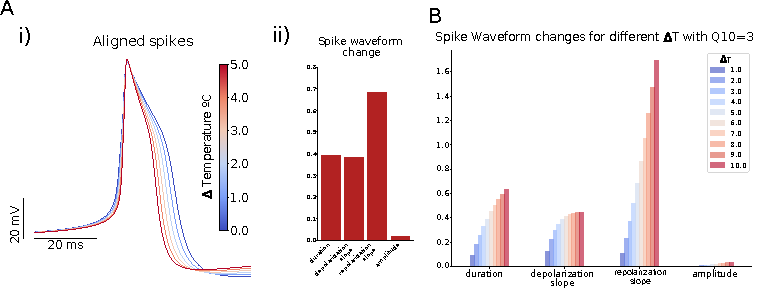
\includegraphics[width=\textwidth]{img/laser/Figure5.pdf}
	\caption{Waveform change in the CGC-model due to $\Delta T$ temperature variation. Panel Ai) shows the spike waveform superposition for distinct $\Delta T$ values. Spikes are aligned to the initial value of each waveform. In panel Aii) the normalized change in the waveform is depicted for all metrics (duration, depolarization and repolarization slopes and amplitude). Panel B shows the change in response to temperature variation from 1 to 10ºC ($Q_{10}=3$) in the normalized metrics.}
	\label{fig:temperature model}
\end{figure}

Figure \ref{fig:temperature model} shows the change in the spike waveform caused by variations in temperature. The $Q_{10}$ factor was added to every dynamical equation in the model (i.e., conductances, activation gates and capacitance, see Sec. \ref{sec:model equations temperature}). In panel A, we show the changes in the waveform for $\Delta T=0-5^{\circ}C$, represented as superimposed waveforms in Ai), and its quantification in Aii) normalized to the maximum, which is analogous to the previous sections (see Figs. \ref{fig:continuous_model} and \ref{fig:continuous_results_panel}): $|max-min|/|max|$. Note how both the spike waveform shape and the quantification of the changes are similar to the experimental results. We can observe changes in duration, depolarization and repolarization slopes, with a very small change in amplitude.
The modulation obtained by combining these parameters was not achieved by tuning them separately. It is important to highlight that as the temperature increased (red lines), the spike got narrower by the corresponding alteration in slopes and duration, which supports the hypothesis that the observed effect in single neurons of \textit{Lymnaea stagnalis} might be, to a large extent, caused by temperature gradient. In panel \ref{fig:temperature model}B, there is a comparison of different temperature changes for the same $Q_{10}$ value in the model. Note that the relation of each parameter to the change in temperature is different, being the repolarization slope the one with the strongest relation, increasing much more rapidly than the duration or the repolarization slope. This points to a main role in the change from some of the channels, especially those that have more tolerance to change. This relation in the repolarization is similar to the comparison of the two neuron types analyzed in the experimental results (Figure \ref{fig:continuous_results_panel}A), where the main difference was present in the repolarization.

\begin{figure}[htb!]
	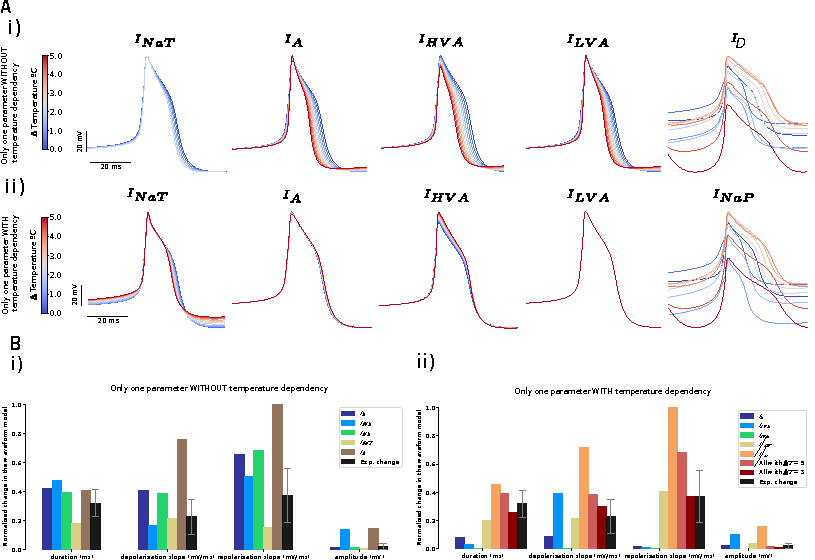
\includegraphics[width=\textwidth]{img/laser/FigureS2.pdf}
	\caption{Simulation of the effect of individual channels on the spike waveform under temperature modulation. Panel A.i) Waveform modulation in the CGC-model excluding temperature dependency in one channel at a time, from left to right: $I_{\textrm{NaT}}$, $I_{A}$, $I_{\textrm{HVA}}$, $I_{\textrm{LVA}}$, $I_{D}$ respectively. Panel A.ii) Waveform modulation in the CGC-model with temperature dependency only in one channel at a time, from left to right: $I_{\textrm{NaT}}$, $I_{A}$, $I_{\textrm{HVA}}$, $I_{\textrm{LVA}}$ and $I_{\textrm{NaP}}$, respectively. Note that  $I_{\textrm{NaP}}$ is not in panel A.i) and neither is $I_{D}$ in A.ii), as for these two particular simulations there was no spike generation. Panels B.i) and B.ii) show the quantification of the waveform change for $\Delta T=5^{\circ}C$ in duration, depolarization slope, repolarization slope and amplitude for all channels in panel A. Both figures include, as reference, the experimental mean and STD (showed in black) and, for case B.ii) (only one channel at a time), the quantification when all channels have the same temperature dependency (all with $\Delta T=5^{\circ}C / 3^{\circ}C$, data used in Fig. \ref{fig:temperature model}) is depicted in light and dark red bars.}
	\label{fig:temperature simulation include exclude}
	
\end{figure}


Analogously to the simulations in the previous sections, we characterized the variations in the waveforms for each individual candidate, varying the temperature only for one ionic-channel at a time. To further explore these candidates and relations, we repeated the model simulation with temperature variations up to 5ºC but also canceling the temperature dependency in one channel at a time. Note that overriding the temperature dependence of some of the channels at a time is only possible in a theoretical environment like this, which allows us to expose the role of each channel in relation to the temperature modulation. Figure \ref{fig:temperature simulation include exclude} shows the result of these simulations. In panel A, there are depicted the waveforms of the model simulation with temperature variations up to 5ºC but canceling the temperature dependency in one channel at a time (i) and describing the dependency of only one channel at a time (ii). In panel B there is a barchart with the metric characterization for each case (with and without temperature dependency) including also the experimental change reference in the dark bars. Panel A.i) shows how the general spike waveform shape was preserved in the range of the tested temperature variations when individually excluding low potassium and calcium currents --$I_{A}$ and $I_{HVA}$ and $I_{LVA}$, respectively-- we were able to simulate the same range as in Fig. \ref{fig:temperature model} of $\Delta T=0-5 ^{\circ}C$. However, when excluding the temperature dependency of $I_{NaT}$, the model could not generate action potentials when raising the temperature for the other channels above $\Delta T=2 ^{\circ}C$, which suggests that $I_{NaT}$ intervention during the temperature modulation is relevant for the action potential generation. This channel presented a non-linear relation between the amplitude and the temperature. It is important also to note that suppression of the temperature dependency in $I_{HVA}$ in Fig. \ref{fig:temperature simulation include exclude}Ai) resulted in a large change in the amplitude (20 mV decrease). This calcium current is needed to preserve the amplitude value while the slopes and duration values change during the temperature increase. The last waveform in that row, $I_D$, displayed a large change in the waveform shape, modifying the duration along with the depolarization currents and thus breaking down the spike. This change corresponds to a strong role in the generation of the action potential for this channel. In the contrary case, in Figure \ref{fig:temperature simulation include exclude}Aii) we observe that the channels with the strongest effect in the model are $I_{NaT}$, $I_{HVA}$ and $I_{NaP}$, since their independent change of temperature produced a notable change in the waveform. Also in opposite to the previous case with temperature dependency, now it is $I_{D}$ the channel that when it is the only one with temperature dependency, there was no spiking activity, and now $I_{NaP}$ displays a large change comparable to the one occurring before with $I_{D}$. In Panel B, we can observe for both cases that no candidate alone could reproduce the observed experimental laser modulation but some channels have a more direct relation to the temperature change such as  $I_{\textrm{LVA}}$ for the repolarization or $I_{D}$ channel, crucial for the spike generation waveform.


Exploring the waveform change during temperature variation showed that the most similar change to the experimental laser modulation was reached in the models with the temperature dependency description in all parameters. We showed that, for most currents as the temperature increases, the experimentally observed modulation relations were maintained, changing in duration and repolarization slope, with a larger change in repolarization slope and a mild change in amplitude. This is also supported by excluding temperature dependency from isolated ion channels and proposing temperature dependency for one channel at a time. Furthermore, it is in agreement with the results of the modeling sweeping the parameter space for distinct candidates without a specific description of the temperature (see Sec. \ref{sec:laser models}), which showed that no modulation of an individual candidate but a combination of them can explain the experimental quantification.

